\documentclass[a4paper,10pt]{article}

\usepackage{ucs}
\usepackage[utf8x]{inputenc}
\usepackage{amsmath}
\usepackage{amssymb}
\usepackage{subfigure}
\usepackage{fontenc}
\usepackage{graphicx}
\usepackage{capt-of}
\usepackage{natbib}
\bibliographystyle{apj.bst}
\usepackage{aas_macros}

\usepackage[dvips]{hyperref}

\date{03/15/15}

\begin{document}
 \section{Introduction}
 \begin{figure}[h!]
  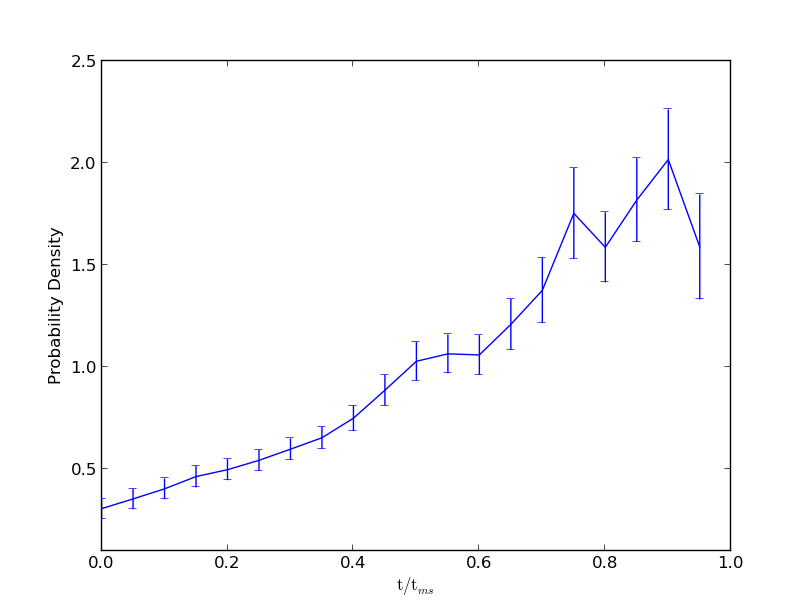
\includegraphics[width=\textwidth]{obsdata}
  \caption{Probability density of galactic stars with masses in the range of $M_{\mathrm{min}}=5\,$M$_{\odot}$ and 
  $M_{\mathrm{max}}=50\,$M$_\odot$ as a function of fractional main sequence age with error bars. Data taken from Fossati et al. (2015) 
  (in prep.)\label{obsdata}}
 \end{figure}

 In a recent study of galactic O and B stars, Fossati et al. found a correlation of fractional main sequence age ($\tau$) and
 the probability density of stars as seen in Figure \ref{obsdata}.  \\
 --First thoughts (Hypothesis)\\
 \subsection{magnitude cut}
 Explanation for magnitude cut \label{magnitudecut}
 \section{Method}
 
 I simulate a synthetic stellar population using three variables to describe every given star: distance from earth ($r$), stellar mass ($M$) 
 and age ($t$). In accordance to the observational data I attempt to model, distance ranges from 0 to $r_{\mathrm{max}}=3\,$kpc and mass
 from $M_{\mathrm{min}}=5\,\mathrm{M}_\odot$ to $M_{\mathrm{max}}=50\,\mathrm{M}_\odot$. Because in first order the main sequence age 
 ($t_{\mathrm{ms}}$) of 
 a star is a strictly monotonic increasing function of $M$ one can define the maximum age for the oldest possible star in my sample to be
 $t_{\mathrm{max}}=t_{\mathrm{ms}}(M_{\mathrm{min}})$. With $M_{\mathrm{min}}=5\,\mathrm{M}_\odot$ and using equation 5 of 
 \citep*{2000MNRAS.315..543H} this translates to $t_{\mathrm{max}}\approx 104\,\mathrm{Myr}$.\\
 
 To formulate a probability density in fractional main sequence age ($\frac{dp}{d\tau}$), I need to know the probability densities for stars in space 
 $\left(\frac{dp}{dV}\right)$, mass 
 $\left(\frac{dp}{dm}\right)$ and age $\left(\frac{dp}{dt}\right)$. In my simulation I assume the stars are uniformly distributed in space. 
 Because of the radial symmetry of the problem, the distribution is solely dependant on the distance from earth,
 
 \begin{equation}
  \frac{dp}{dV}=\frac{1}{V_{\mathrm{tot}}}=\frac{1}{\frac43\cdot\pi\cdot r_{\mathrm{max}}^3}.
  \label{dpdV}
 \end{equation}
 
  I assume the stars are distributed in mass according to the Salpeter Initial Mass Function (IMF):
 $\frac{dp}{dM}=A\cdot M^{-2.35}$ \citep*{1955ApJ...121..161S}. Because the IMF follows an inverse power law, I use a logarithmic mass axis.
 Because of that I need to convert the IMF to a logarithmic binning using $d\log M = \frac{dM}{M\ln 10}$
 
 \begin{equation}
  \frac{dp}{d\log M}=\ln 10 \cdot A\cdot M^{-1.35},
 \end{equation}
 
 Where A is a normalization factor, that follows from: 
 
 \begin{equation}
  1=\int_{M_{\mathrm{min}}}^{M_{\mathrm{max}}}A\cdot M^{-2.35} dM =\left[ -1.35\cdot A\cdot M^{-1.35}\right]_{M_{\mathrm{min}}}^{M_{\mathrm{max}}},
 \end{equation}
 
 \begin{equation}
  A= \frac{1.35}{M_{\mathrm{min}}^{-1.35}-M_{\mathrm{max}}^{-1.35}}.
 \end{equation}
 
 I assume a constant star formation rate, so the probability density in age is $\frac{dp}{dt}=\frac{1}{t_{\mathrm{ms}}}$. 
 The age axis is also defined logarithmic to make sure massive stars with small $t_{\mathrm{ms}}$ are correctly represented.
 Because of this I need to find $\frac{dp}{d\log t}$ using $d\log t=\frac{dt}{t \ln 10}$; 

 \begin{equation}
  \frac{dp}{d\log t}=\frac{t\ln 10}{t_{\mathrm{ms}}}.
 \end{equation}

 With this information I can formulate the overall probability density function (PDF) for the stars in my sample with regard to $\tau$
 
 \begin{equation}
  \frac{dp}{d\tau}=\frac{dp}{dV}dV \cdot \frac{dp}{d\log t}d\log t \cdot \frac{dp}{d\log M}d\log M\cdot \frac{1}{d\tau}.
 \end{equation}
  
 
 To implement a magnitude cut I need to find the visual magnitude (V) for any given star. 
 The first step is to use analytical formulations derived from a stellar evolution model by \citet{2000MNRAS.315..543H} which approximates the
 stellar evolution as a function of initial mass ($M_{\mathrm{ini}}$), fractional main sequence age ($\tau$) and metalicity (Z).
 To do this, I need to find $\tau$. Equation 5 of \citep{2000MNRAS.315..543H} gives me the main sequence age for any given mass
 $t_{\mathrm{ms}}(M)$ and $\tau$ then becomes: $\tau(M)=\frac{t}{t_{\mathrm{ms}}(M)}$. I use Z=0.02 for all stars to simulate a metalicity
 similar to that of our sun according to \citet*{1998SSRv...85..161G}.
 I then use Equation 12 and 13 from the same paper to compute luminosity (L) and radius (R) for stars on the main sequence\footnote{
 \citet{2000MNRAS.315..543H} cites \citet*{1996MNRAS.281..257T} for Zero Age Mainsequence Radii and Luminosities. 
 In Equation 1 of the cited paper there is a typo, where: $\gamma + M^3$ has to be $\gamma \cdot M^3$.}. \\
 
 Figure \ref{lumiradius} shows a Hertzsprung Russel Diagram (HRD) for five different stars on their main sequence based on the evolutionary
 model of \citet{2000MNRAS.315..543H}. To obtain temperature (T) I use the following equation with $\sigma$ being the Stefan-Boltzmann-Constant:
 
 \begin{equation}
  T=\sqrt[4]{L/(\sigma 4 \pi R^2)}.
 \end{equation}
 
  \begin{figure}[h!]
  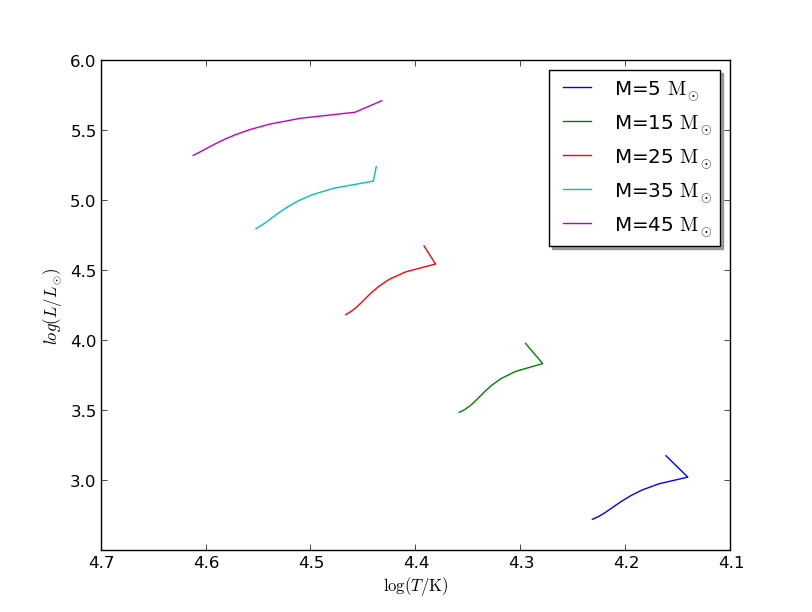
\includegraphics[width=\textwidth]{lumiradius}
  \caption{HRD for five different stars on their main sequence based on the evolutionary model of \citet{2000MNRAS.315..543H} \label{lumiradius}}
 \end{figure}
 

 With distance, mass, age, fractional main sequence age, luminosity and radius I can  
 compute the apparent magnitudes using the following equations:
 
 \begin{equation}
  M_{\mathrm{V}}=V-5\cdot\log(r)+5-A(r),
  \label{MV}
 \end{equation}
 
 \begin{equation}
  M_{\mathrm{bol}}=M_{\mathrm{V}}+BC,
  \label{Mbol}
 \end{equation}
 
 \begin{equation}
  \log(L/\mathrm{L}_\odot)=0.4\cdot(4.72-M_{\mathrm{bol}}).
  \label{LMbol}
 \end{equation}
 
 Where $M_{\mathrm{V}}$ is the absolute visual magnitude, $\log(r)$ is the logarithm to base ten of the distance from earth. $A(r)$ is the 
 reddening, $M_{\mathrm{bol}}$ is the absolute bolometric magnitude and $BC$ is the Bolometric Correction from a model by 
 \citet*{1996ApJ...469..355F}. Using equations \ref{MV}, \ref{Mbol} and \ref{LMbol} I can compute the apparent visual magnitude $V$:
 
 \begin{equation}
  V=5\cdot\log(r)-5+A(r)+4.72-\frac{\log(L/\mathrm{L}_\odot)}{0.4}-BC.
 \end{equation}
 
 To get a rough approximation for reddening, I use \citet*[Figure 9]{2005AJ....130..659A}. I linearly interpolate the three intervals between:
 $r=0\,$kpc, $A=0$; $r=1\,$kpc, $A=0.9$; $r=2\,$kpc, $A=2.25$ and $r=3\,$kpc, $A=3.273$. 
 
 
 \newpage
 \section{Tests}
 I conducted a few consistency and numerical tests.:
 
 \subsection{consistency checks}
 
 \subsection{numerical tests}
 \begin{figure}[h!]
  \begin{minipage}{0.49\textwidth}
   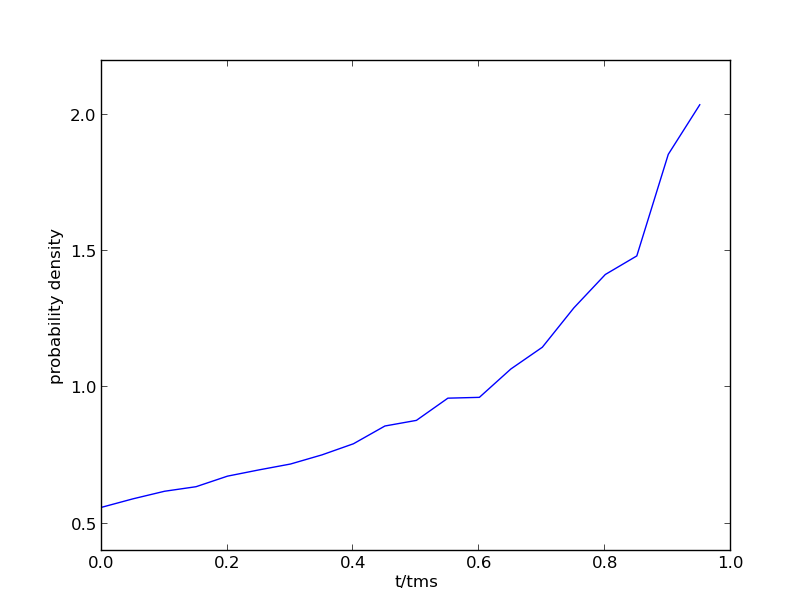
\includegraphics[width=\textwidth]{100-100-100}
  \end{minipage}
  \begin{minipage}{0.49\textwidth}
   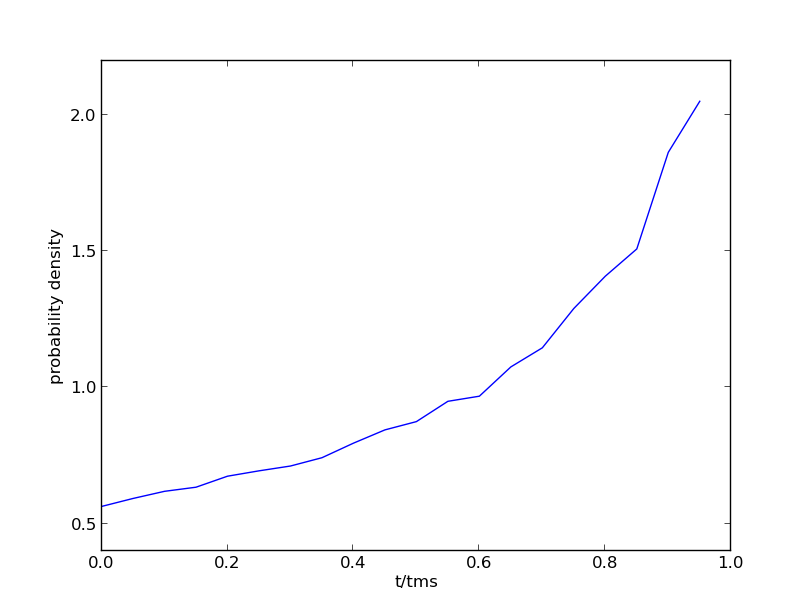
\includegraphics[width=\textwidth]{10-100-100}
  \end{minipage}
  \begin{minipage}{0.49\textwidth}
   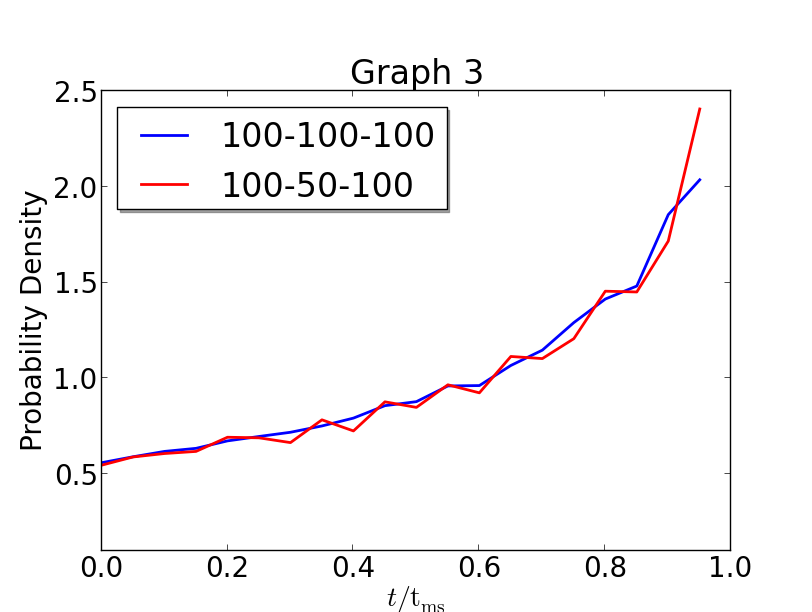
\includegraphics[width=\textwidth]{100-50-100}
  \end{minipage}
  \begin{minipage}{0.49\textwidth}
   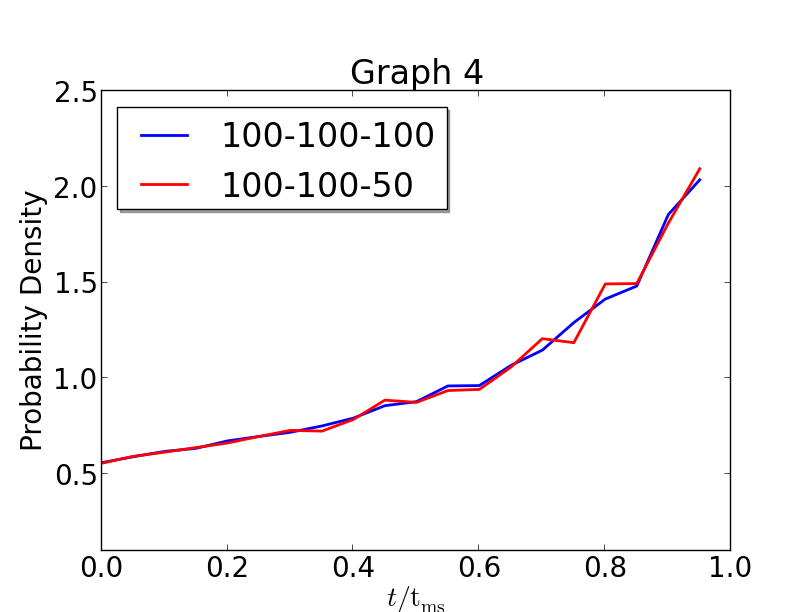
\includegraphics[width=\textwidth]{100-100-50}
  \end{minipage}
   \caption{PDF for all stars in my sample with a magnitude cut at V=9 with different binnings.
   The legend shows the binning of each line. The first value being distance, the second being mass and the third being age.\label{binnings}}
 \end{figure}
 
 Figure \ref{binnings} shows the PDF for all stars in my sample with a magnitude cut at V=9 in four graphs. 
 Graph 1 shows both the function with a resolution of 100-100-100 in distance-mass-age and the final results without noise for reference. 
 One can see from this
 graph that with this resolution there is noise that needs to be eliminated. 
 To understand what variables play the biggest part in creating this noise, in Graphs 2, 3 and 4 I change the resolution of a select 
 variable and compare the resulting curve to the curve of 100-100-100 resolution.\\
 
 In Graph 2 one can see, that even though I cut the resolution of distance by one order of magnitude, the curves only deviate very little. This
 tells me, that distance will be very robust to a low resolution. Graphs 3 and 4, even though I only cut the resolution in half, both 
 show a significant increase in noise, Graph 3 showing the greatest deviation from the reference-curve. Using these results, I determine 
 a binning of 100-1500-750 to yield an appropriate resolution to maximize accuracy and minimize computing time.
 
 \newpage
 \section{Results}
 \begin{figure}[h!]
   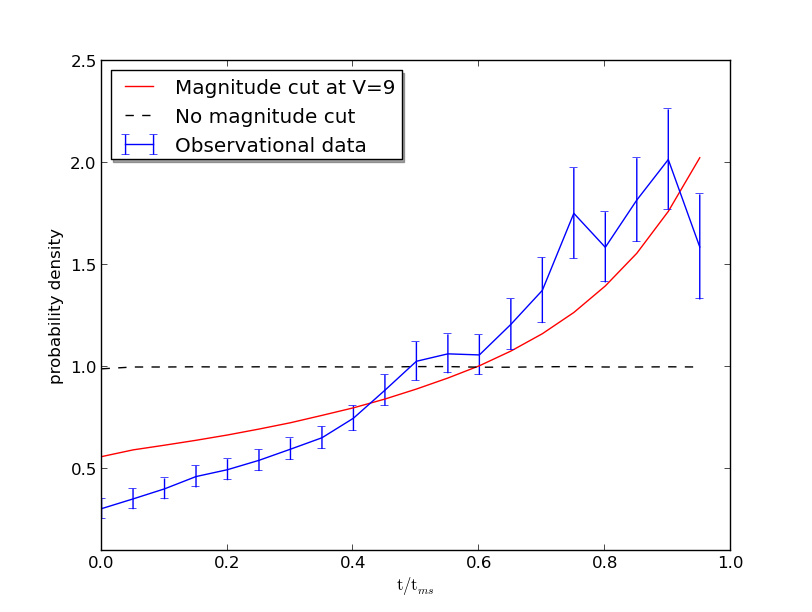
\includegraphics[width=\textwidth]{plot1}
   \caption{PDF of volume limited sample, with magnitude cut at V=9 (red line), PDF without magnitude cut
   (dashed line) and observational data with error bars (blue line). All computed data is obtained using a binning of 100-1500-750
   in distance-mass-age. The observational data is taken from Fossati et al., 2015 (in prep.).\label{all3}}
 \end{figure}
 
 Figure \ref{all3} shows the PDF with magnitude cut at V=9, PDF without magnitude cut and observational data with error bars.
 The PDF without magnitude cut shows, that the stars are uniformly distributed in $\tau$. This was expected,
 because the simluation assumes a constant star formation rate.\\
 
 Introducing a magnitude cut produces a similar trend to the one observed in the observational data. Because V is a monotonic decreasing
 function in age, there will be more old stars below the magnitude cut, than young stars. Figure \ref{magage} shows
 V as a function of fractional main sequence age for five different stars at a distance of 1$\,$kpc based on the evolutionary model of 
 \citet{2000MNRAS.315..543H}. At Zero Age Main Sequence (ZAMS) stars with $r=1\,$kpc $M>15\mathrm{M}_\odot$ fall below the magnitude cut at 
 $V=9$. At terminal age main sequence (TAMS) however, every star in a distance of $r=1\,$kpc and $M>5\,$M$_\odot$ falls below this cut.\\
 \begin{figure}
  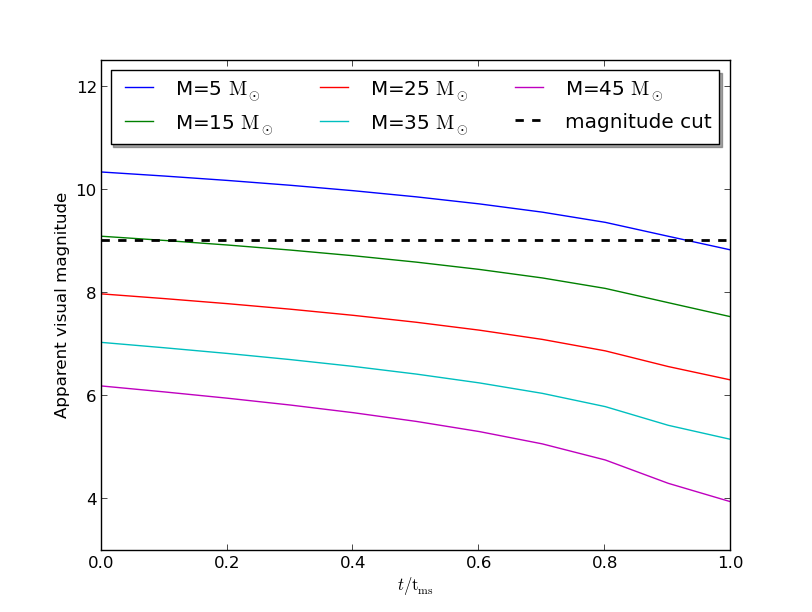
\includegraphics[width=\textwidth]{magage}
  \caption{V as a function of fractional main sequence age for five different stars at a distance of 1$\,$kpc based on the evolutionary model 
  of \citet{2000MNRAS.315..543H} The dashed line shows the magnitude cut I implemented.\label{magage}}
 \end{figure}

 There are a lot of things, that can still be implemented:\\
 \begin{itemize}
  \item The stars are distributed homogenously in a sphere of 3$\,$kpc radius. To make it more accurate one could model take into account the 
  thickness of the galactic disk, which is smaller, than 3$\,$kpc. 
  \item The program does not take into account binary stars. This possibly has a major effect, because most massive stars are in binary
  systems \citep{2012Sci...337..444S}
  \item From observations we know, that we live in a part of the galaxy with little star formation.  
  The density of young open starclusters increases the farther you move away from the solar system. Figure \ref{clusters} shows open 
  starclusters in our galaxy with distance modulus vs log($t$/yr). The black line represents the age of the oldest possible star in 
  my sample. Starclusters below this limit show a trend, where young clusters are farther away, than old ones.
  \item My model for reddening is only an approximation. It does not take into account density fluctuations in the interstellar medium. 
  The effects of which can be seen in figures \textbf{reference to diffmag}.
 \end{itemize}
 \begin{figure}[h!]
  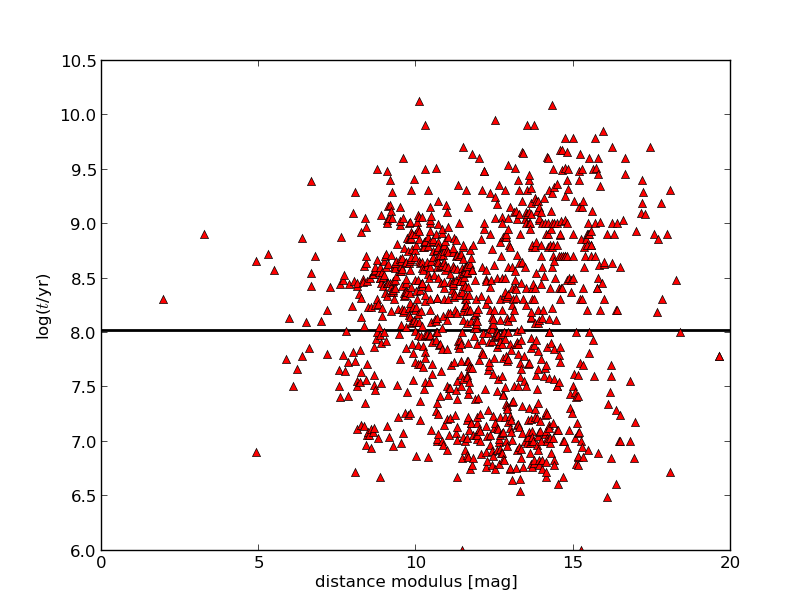
\includegraphics[width=\textwidth]{clusters}
  \caption{Open starclusters in our galaxy with distance modulus vs log($t$/yr). The black line represents the age of the oldest possible
  star in my sample. ($t_{\mathrm{ms}}(M_{\mathrm{min}})=104\,$Myr) \textbf{citation} \label{clusters}}
 \end{figure}

 \newpage
 \section{Conclusions}
 I modeled a stellar population for stars on their main sequence of masses between $M=5\,$M$_\odot$ and $M=50\,$M$_\odot$ and a distance of 
 $r\le 3\,$kpc. I defined the probability density function (PDF) with regard to the fractional main sequence age $\frac{dp}{d\tau}$ using 
 the PDFs for space $\frac{dp}{dV}$, mass $\frac{dp}{dM}$ and age $\frac{dp}{dt}$. I implemented
 analytical formulations derived from a stellar evolution model by \citet{2000MNRAS.315..543H} to find the apparent visual magnitudes.
 I modeled the magnitude limited PDF and found, that it matches the trend of the observational data very well.\\
 With this I proved, that you do indeed expect a trend similar to the one found in Figure \ref{obsdata} taking into account modern stellar 
 evolution models.\\
 
 In the future this work can be used to simulate a more detailed model and explain the deviations, that occur in this simulation.
 
 
 \bibliography{adssample}
\end{document}
